\documentclass[11pt]{article}
\usepackage{amsmath, amssymb, amscd, amsthm, amsfonts}
\usepackage{graphicx}
\usepackage{hyperref}
\usepackage{physics}
\usepackage{listings}

\hypersetup{
    colorlinks=true,
    linkcolor=blue,
    filecolor=magenta,      
    urlcolor=blue,
    }

\DeclareMathOperator{\E}{\mathbb{E}}
\DeclareMathOperator{\Var}{\mathbb{V}}
\DeclareMathOperator{\Prob}{\mathbb{P}}
\DeclareMathOperator{\Real}{\mathbb{R}}
\DeclareMathOperator*{\argmax}{arg\,max}
\DeclareMathOperator*{\argmin}{arg\,min}

\oddsidemargin 0pt
\evensidemargin 0pt
\marginparwidth 40pt
\marginparsep 10pt
\topmargin -20pt
\headsep 10pt
\textheight 8.7in
\textwidth 6.65in
\linespread{1.2}
\setlength{\parindent}{0em}

\title{DATA 557: Applied Statistics and Experimental Design \\ Homework 1}
\author{Abhishek Saini}
\date{January 2022}

\newtheorem{theorem}{Theorem}
\newtheorem{lemma}[theorem]{Lemma}
\newtheorem{conjecture}[theorem]{Conjecture}

\newcommand{\rr}{\mathbb{R}}

\newcommand{\al}{\alpha}
\DeclareMathOperator{\conv}{conv}
\DeclareMathOperator{\aff}{aff}

\DeclareUnicodeCharacter{2212}{-}

\begin{document}

\maketitle

\section*{Question 1}
Suppose that you flip a coin 40 times and count the number of heads.

\subsection*{1.1. What is the distribution of the number of heads assuming the coin is fair?}
Since each coin toss is independent and identically distributed Bernoulli trial and the coin is fair, the distribution of the number of heads is a Binomial distribution with $n = 40$ and $p=0.5$

\subsection*{1.2. The sample proportion of heads has an approximately normal distribution. What are the mean and standard deviation of this distribution assuming the coin is fair?}
The sample proportion is the random variable $S = \frac{\sum_{i=1}^{40}X_i} {40} $. \\
Its mean $\mu = p = 0.5$ and standard deviation $\sigma = \sqrt{p(1-p)/n} = \sqrt{\frac{0.5\times0.5}{40}} \approx 0.079$

\subsection*{1.3. Define the Z-statistic for conducting a test of the null hypothesis that the coin is fair (i.e., has probability of a head equal to 0.5).}
We can define the Z-statistic as:
\begin{equation*}
    Z = \frac{S-\mu}{\sigma} = \frac{S-0.5}{\sqrt{0.00625}} \approx \frac{S-0.5}{0.079}
\end{equation*}

\subsection*{1.4. Suppose the experiment results in 15 heads and 25 tails. Conduct a test of the null hypothesis with type I error probability 0.05 using the normal approximation. State the Z statistic, the p-value, and the conclusion of the test (do you reject the null hypothesis or not).}
\begin{equation*}
    Z = \frac{\frac{15}{40} - 0.5}{\sqrt{0.00625}} = -1.581139
\end{equation*}
This gives a p value 0.1138463 under the normal approximation. We conclude that we do not have sufficient information to reject the null hypothesis.
\begin{lstlisting}[language=R]
> p_val = 2*pnorm(Z)
> p_val
[1] 0.1138463
\end{lstlisting}

\subsection*{1.5. If you had decided to use a type I error probability of 0.1 instead of 0.05 would your conclusion be different? Explain.}
Even with type I error probability of 0.1, we would not be able to reject the null because the p value approximated under the normal distribution is 0.1138463 greater than 0.1, the decision boundary for our test.

\subsection*{1.6. Calculate the p-value using the binomial distribution. Do you reach the same conclusion with the binomial distribution as with the normal approximation?}
On calculating the p-value using the binomial distribution, we get a p-value less than 0.1 and hence we reject the null hypothesis. We reach a different conclusion with the binomial distribution.
\begin{lstlisting}[language=R]
> # binomial p value
> rejection_region = c(0:14, 26:40)
> sum(dbinom(rejection_region, size=n, p=mean))
[1] 0.08069047
\end{lstlisting}


\subsection*{1.7. Calculate a 95\% confidence interval for the probability of a head using the normal approximation. Does the confidence interval include the value 0.5?}
95\% confidence interval lies between $(S - 1.96 SE, S + 1.96 SE) = (0.375-1.96\times0.0765, 0.375+1.96\times0.0765) = (0.2249688, 0.5250312)$ and this includes $0.5$

\begin{lstlisting}[language=R]
> # 95% confidence interval
> std_err = sqrt(S*(1-S)/n)
> c(S-1.96*std_err, S+1.96*std_err)
[1] 0.2249688 0.5250312
\end{lstlisting}

\subsection*{1.8. Calculate a 90\% confidence interval for the probability of a head using the normal approximation. How does it compare to the 95\% confidence interval?}
The 90\% confidence interval turns out to be (0.2490809, 0.5009191). It is smaller than the 95\% confidence interval but still includes $0.5$.
\begin{lstlisting}[language=R]
> # 90% confidence interval
> c(S-1.645*std_err, S+1.645*std_err)
[1] 0.2490809 0.5009191
\end{lstlisting}

\section*{Question 2}
A study is done to determine if enhanced seatbelt enforcement has an effect on the proportion of drivers wearing seatbelts. Prior to the intervention (enhanced enforcement) the proportion of drivers wearing their seatbelt was $0.7$. The researcher wishes to test the null hypothesis that the proportion of drivers wearing their seatbelt after the intervention is equal to $0.7$ (i.e., unchanged from before). The alternative hypothesis is that the proportion of drivers wearing their seatbelt is not equal to $0.7$ (either $< 0.7$ or $> 0.7$). After the intervention, a random sample of $400$ drivers was selected and the number of drivers wearing their seatbelt was found to be $305$.

\subsection*{2.1. Calculate the estimated standard error of the proportion of drivers wearing seatbelts after the intervention.}
The estimated standard error of the proportion of drivers wearing seatbelts after the intervention is given by $\sqrt{\hat{p}(1-\hat{p})/n} = \sqrt{\frac{305}{400}(1-\frac{305}{400})/400} = 0.02127756$
\begin{lstlisting}[language=R]
> # estimated standard error
> std_error = sqrt(S*(1-S)/n)
> std_error
[1] 0.02127756
\end{lstlisting}

\subsection*{2.2. Calculate a 95\% confidence interval for the proportion of drivers wearing seatbelts after the intervention. What conclusion would you draw based on the confidence interval?}
The $95\%$ confidence interval is $(0.720796, 0.804204)$. We reject the null hypothesis because $0.7$ is outside the confidence interval. 
\begin{lstlisting}[language=R]
> # 95% confidence interval
> c(S-1.96*std_error, S+1.96*std_error)
[1] 0.720796 0.804204
\end{lstlisting}


\subsection*{2.3. Conduct a test of the null hypothesis with type I error probability 0.05 using the normal approximation. Should the null hypothesis be rejected? How does your conclusion compare to the conclusion from the confidence interval?}
The p value is 0.006 and below our threshold for type I error probability. Hence, we should reject the null hypothesis. The conclusion is the same as we got from using confidence intervals.
\begin{lstlisting}[language=R]
> # p value using normal approximation
> p_val = 2*(1-pnorm(Z))
> p_val
[1] 0.006377301
\end{lstlisting}

\subsection*{2.4. Calculate the approximate p-value using the normal approximation and the exact p-value using the binomial distribution. Are the two p-values very different?}
The p value using normal approximation is 0.006 and using binomial distribution is 0.002 and their absolute difference is low compared to the type I error probability.
\begin{lstlisting}
> # p value using binomial distribution
> rejection_region = c(0:94, 306:400)
> sum(dbinom(rejection_region, size=n, p=p))
[1] 0.00226463
\end{lstlisting}


\subsection*{2.5. Calculate the power of the test to detect the alternative hypothesis that the proportion of drivers wearing their seatbelts after the intervention is equal to 0.8.}
Power = $P(Reject\, H_0| alternate \,\, hypothesis) = P(Reject\, H_0| p=0.8)$
For type I error probability of 0.05 the rejection region is number of drivers wearing seatbelts $<$ 105 and number of drivers wearing seatbelts $>$ 295 on calculating the p value using the binomial distribution.\\
The power turns out to be 0.9985187.
\begin{lstlisting}[language=R]
> r = 104
> rejection_region = c(0:r, (400-r):400)
> sum(dbinom(rejection_region, size=n, p=0.8))
[1] 0.9985187
\end{lstlisting}


\section*{Question 3}

\subsection*{3.1. Create a histogram of the IQ variable. Is the distribution approximately normal?}
The histogram plotted is shown below. This doesn't look like a normal distribution because of the sharp increase in IQ from 70 to 80. 

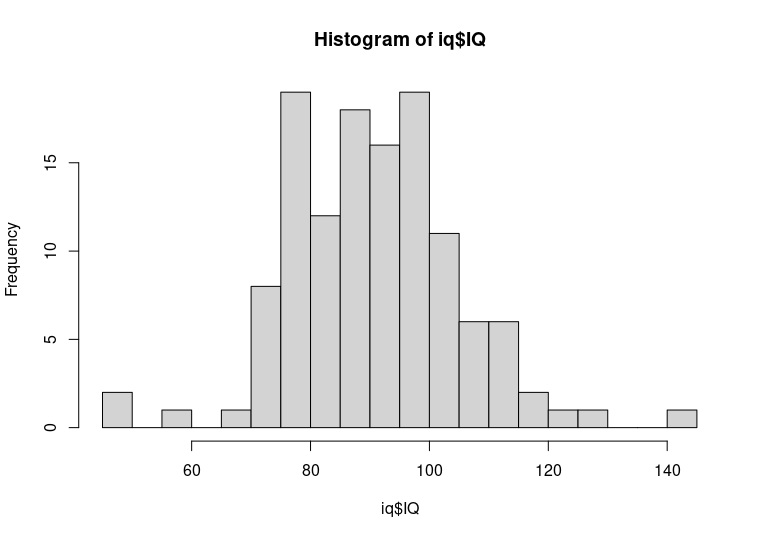
\includegraphics[width=150mm]{Rplot01.png}

\subsection*{3.2. Calculate the sample mean and sample SD of IQ. How do they compare numerically to the US population values?}
The sample mean is 91.08065 and the sample SD is 14.40393. According to this \href{https://www.ncbi.nlm.nih.gov/pmc/articles/PMC4603674/}{article}, their estimated US population mean is higher at 100 and standard deviation is 15. The difference may or may not be statistically significant.
\begin{lstlisting}[language=R]
> mean(iq$IQ)
[1] 91.08065
> sd(iq$IQ)
[1] 14.40393
\end{lstlisting}

\subsection*{3.3. Test the null hypothesis that the mean IQ score in the community is equal to 100 using the 2-sided 1-sample t-test with a significance level of 0.05. State the value of the test statistic and whether or not you reject the null hypothesis at significance level 0.05.}
The test statistic for the 2-sided 1-sample t-test is given as
\begin{equation*}
\abs{Z} = \frac{\abs{\hat{X} - \mu_0}}{s/\sqrt{n}} = 6.895462    
\end{equation*}
We should reject the null hypothesis because the test statistic is greater than the critical value of the $t_{123,0.05} \approx 1.98$ 


\begin{lstlisting}[language=R]
> # hypothesis test: H0 is that the mean = 100
> Z = abs(mean(iq$IQ) - 100)/(sd(iq$IQ)/sqrt(length(iq$IQ)));Z
[1] 6.895462
\end{lstlisting}

\subsection*{3.4. Give the p-value for the test in the previous question. State the interpretation of the p-value.}
The p-value for the test is 2.486475e-10. This means that the probability, under the null hypothesis, of seeing an observation as extreme or more than what we observed is 2.486475e-10.
\begin{lstlisting}[language=R]
> # p-value calculation 
> p_val = 2*pt(Z, 123, lower.tail = FALSE); p_val
[1] 2.486475e-10
\end{lstlisting}


\subsection*{3.5. Compute a 95\% confidence interval for the mean IQ. Do the confidence interval and hypothesis test give results that agree or conflict with each other? Explain.}
The 95\% confidence interval is between $\hat{X} - 1.98 \times SE$ and $\hat{X} + 1.98 \times SE = (88.51949, 93.64180)$ and it doesn't contain 100. We get the same result from confidence interval and hypothesis test because the result is very extreme. 
\begin{lstlisting}[language=R]
> # 95% confidence interval
> c(mean(iq$IQ) - 1.98*std_error, mean(iq$IQ) + 1.98*std_error)
[1] 88.51949 93.64180
\end{lstlisting}


\subsection*{3.6. Repeat the hypothesis test and confidence interval using a significance level of 0.01 and a 99\% confidence interval.}
We should reject the null hypothesis because the test statistic is greater than the critical value of the $t_{123,0.01} \approx 2.62$.
\\
The 99\% confidence interval is between $\hat{X} - 2.62 \times SE$ and $\hat{X} + 2.62 \times SE = (87.69165, 94.46964)$
\begin{lstlisting}[language=R]
> # 99% confidence interval
> c(mean(iq$IQ) - 2.62*std_error, mean(iq$IQ) + 2.62*std_error)
[1] 87.69165 94.46964
\end{lstlisting}

\end{document}